\documentclass[letter,11pt]{article}
%\documentclass[letter,twoside,11pt]{article}

\usepackage[spanish,es-nodecimaldot]{babel}
\usepackage[utf8]{inputenc}

\usepackage{lmodern}
\usepackage[T1]{fontenc}
\usepackage{textcomp}

\usepackage{framed}
\usepackage[svgnames]{xcolor}
\colorlet{shadecolor}{Gainsboro!50}

\usepackage{graphicx}
\usepackage{pstricks}

\usepackage{anysize}
\marginsize{3cm}{2cm}{2cm}{3cm}

\usepackage{amsmath}
\usepackage{array}
\usepackage{alltt}

\usepackage{fancyhdr}
\usepackage{lastpage}
\pagestyle{fancy}
\fancyhf{}
\fancyhead[LE,RO]{Laboratorio de Física Básica I}
\fancyfoot[CO,CE]{\thepage\ de \pageref{LastPage}}

\special{papersize=215.9mm,279.4mm}

\usepackage[
    pdfauthor={Carlos Eduardo Caballero Burgoa},%
    pdftitle={Laboratorio de Física Básica I},%
    pdfsubject={Energía},%
    colorlinks,%
    citecolor=black,%
    filecolor=black,%
    linkcolor=black,%
    urlcolor=black,
    breaklinks]{hyperref}
\usepackage{breakurl}

\newcommand{\blankpage}{
\newpage
\thispagestyle{empty}
\mbox{}
\newpage
}

\renewcommand{\arraystretch}{1.2}

\begin{document}

\begin{titlepage}
\begin{center}
{\Large UNIVERSIDAD MAYOR DE SAN SIMÓN}\\
\vspace*{0.15cm}
{\large FACULTAD DE CIENCIAS Y TECNOLOGÍA}\\
\vspace*{0.10cm}
DEPARTAMENTO DE FÍSICA\\
\vspace*{3.0cm}
{\Large \textbf{LABORATORIO DE FÍSICA BÁSICA I}}\\
\vspace*{0.3cm}
{\Large \textbf{PRACTICA No. 8}}\\
\vspace*{3.5cm}
{\Large \textbf{ENERGÍA}}\\
\end{center}

\vspace*{7.4cm}
\leftskip=7.95cm
\noindent
\textbf{Estudiante:}\\
Caballero Burgoa, Carlos Eduardo.\\
\newline
\textbf{Docente:}\\
Msc. Guzmán Saavedra, Rocio.\\
\newline
\textbf{Grupo:} N5.\\
\textbf{Fecha de realización:} 12 de Enero del 2021.\\
\textbf{Fecha de entrega:} 12 de Enero del 2021.\\

\end{titlepage}

\blankpage

\section{Objetivo}
Verificar dentro del marco experimental la conservación de la energía.

\section{Marco teórico}

\begin{figure}[!h]
\centering
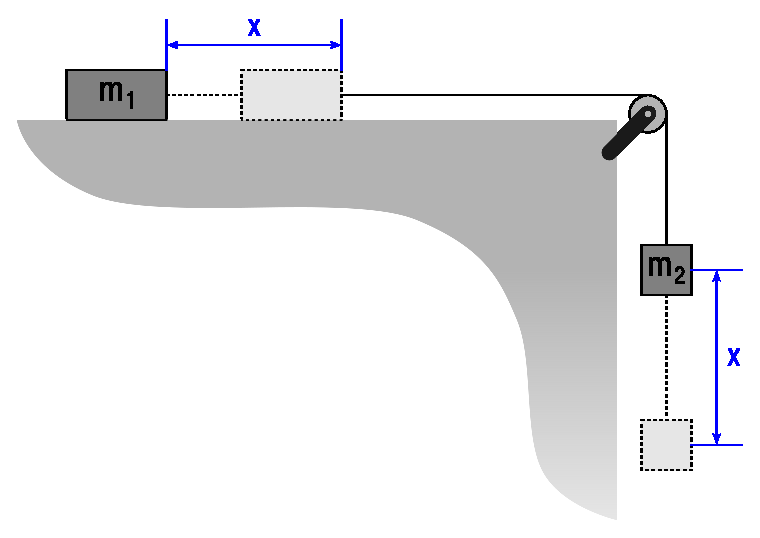
\includegraphics[scale=0.60]{resources/figura1.eps}
\caption{Sistema de dos bloques}
\label{figura1}
\end{figure}

La energía inicial total $E_i$ del sistema de la figura \ref{figura1}
(inicialmente en reposo) formado por las masas $m_1$ y $m_2$, esta compuesta por
la energía potencial gravitatoria $E_p$. La energía final $E_f$ total del
sistema esta formada por la energía potencial gravitatoria $E_p$ y la energía
cinética de translación $E_T$ de ambas masas, el balance de energía requiere
considerar el calor $Q$ generado por la fuerza de fricción, de modo que:

\begin{equation*}
    E_i = E_f + Q
\end{equation*}

Donde:

\begin{equation*}
    E_i = m_1 g h_{1i} + m_2 g h_{2i}
\end{equation*}

\begin{equation*}
    E_f = m_1 g h_{1f} + m_2 g h_{2f} + \frac{1}{2} ( m_1 + m_2 ) v_f^2
\end{equation*}

\begin{equation*}
    Q = | \mu m_2 g \Delta x |
\end{equation*}

Donde $h$ es la altura de cada masa respecto de un nivel de referencia, $v$ la
velocidad de las masas y $\Delta x$ el desplazamiento de $m_2$.

\section{Materiales}
\begin{itemize}
    \item Simulador «PhET Interactive Simulations» Pista de patinar ``Energía''.
\end{itemize}

\section{Procedimiento}
A continuación se describe el procedimiento experimental que se llevará a
cabo.

\begin{enumerate}
\item Haciendo uso del simulador, acomodar la pista para el desplazamiento del
    patinador (ver figura \ref{pistas}), y tomar los datos de altura ($h$),
    velocidad ($v$), energía potencial ($E_p$), energía cinética ($E_c$), y
    energía total ($E_T$), para diversos puntos del recorrido.
\item Graficar los datos tomados tal que pueda verse la relación funcional entre
    estas variables.
\item Comentar la gráfica de la energía mecánica en función de la altura.
\end{enumerate}

\vspace*{2.5cm}
\begin{figure}[!h]
\centering
\includegraphics[scale=0.30]{resources/pistas.eps}
\caption{Pistas configuradas en el simulador}
\label{pistas}
\end{figure}
\section{Tablas de datos y resultados}

\subsubsection{Datos obtenidos}

\begin{center}
\begin{tabular}{|c|>{\centering}m{2.0cm}<{\centering}
                  |>{\centering}m{2.0cm}<{\centering}
                  |>{\centering}m{2.0cm}<{\centering}
                  |>{\centering}m{2.0cm}<{\centering}
                  |>{\centering}m{2.0cm}<{\centering}|}
\hline
\multicolumn{6}{|c|}{\textbf{Tabla \#1: Energía-Altura}} \\
\hline
$i$ & $h_i [m]$ & $v_i [m/s]$ & $E_{pi} [J]$ & $E_{ci} [J]$ & $E [J]$ \tabularnewline \hline
  1 & 3.74 & 4.70 & 734 & 221 & 1028 \tabularnewline \hline
  2 & 3.29 & 5.57 & 645 & 309 & 1028 \tabularnewline \hline
  3 & 2.77 & 6.42 & 543 & 412 & 1028 \tabularnewline \hline
  4 & 2.18 & 7.26 & 428 & 527 & 1028 \tabularnewline \hline
  5 & 1.55 & 8.07 & 303 & 651 & 1028 \tabularnewline \hline
  6 & 0.89 & 8.83 & 175 & 780 & 1028 \tabularnewline \hline
  7 & 0.30 & 9.47 &  59 & 896 & 1028 \tabularnewline \hline
  8 & 0.12 & 9.65 &  23 & 931 & 1028 \tabularnewline \hline
  9 & 0.44 & 9.32 &  87 & 868 & 1028 \tabularnewline \hline
 10 & 1.07 & 8.64 & 209 & 746 & 1028 \tabularnewline \hline
 11 & 1.72 & 7.86 & 337 & 618 & 1028 \tabularnewline \hline
 12 & 2.34 & 7.04 & 459 & 495 & 1028 \tabularnewline \hline
 13 & 2.91 & 6.20 & 571 & 384 & 1028 \tabularnewline \hline
 14 & 3.42 & 5.34 & 670 & 285 & 1028 \tabularnewline \hline
 15 & 3.85 & 4.48 & 754 & 200 & 1028 \tabularnewline \hline
 16 & 4.21 & 3.61 & 825 & 130 & 1028 \tabularnewline \hline
 17 & 4.49 & 2.74 & 880 &  75 & 1028 \tabularnewline \hline
 18 & 4.69 & 1.87 & 920 &  34 & 1028 \tabularnewline \hline
 19 & 4.84 & 0.73 & 950 &   5 & 1028 \tabularnewline \hline
 20 & 4.87 & 0.14 & 955 &   0 & 1028 \tabularnewline \hline
\end{tabular}

\begin{tabular}{|c|>{\centering}m{2.0cm}<{\centering}
                  |>{\centering}m{2.0cm}<{\centering}
                  |>{\centering}m{2.0cm}<{\centering}
                  |>{\centering}m{2.0cm}<{\centering}
                  |>{\centering}m{2.0cm}<{\centering}|}
\hline
\multicolumn{6}{|c|}{\textbf{Tabla \#2: Energía-Altura}} \\
\hline
$i$ & $h_i [m]$ & $v_i [m/s]$ & $E_{pi} [J]$ & $E_{ci} [J]$ & $E [J]$ \tabularnewline \hline
  1 & 5.09 & 0.10 & 3742 &    0 & 6743 \tabularnewline \hline
  2 & 4.95 & 1.66 & 3639 &  103 & 6743 \tabularnewline \hline
  3 & 4.76 & 2.53 & 3502 &  240 & 6743 \tabularnewline \hline
  4 & 4.51 & 3.36 & 3319 &  422 & 6743 \tabularnewline \hline
  5 & 4.23 & 4.09 & 3115 &  627 & 6743 \tabularnewline \hline
  6 & 4.02 & 4.57 & 2960 &  782 & 6743 \tabularnewline \hline
  7 & 4.01 & 4.60 & 2947 &  795 & 6743 \tabularnewline \hline
  8 & 4.11 & 4.37 & 3026 &  716 & 6743 \tabularnewline \hline
  9 & 4.26 & 4.03 & 3132 &  610 & 6743 \tabularnewline \hline
 10 & 4.39 & 3.69 & 3231 &  511 & 6743 \tabularnewline \hline
 11 & 4.48 & 3.44 & 3298 &  444 & 6743 \tabularnewline \hline
 12 & 4.50 & 3.40 & 3309 &  433 & 6743 \tabularnewline \hline
 13 & 4.41 & 3.65 & 3244 &  498 & 6743 \tabularnewline \hline
 14 & 4.21 & 4.14 & 3099 &  643 & 6743 \tabularnewline \hline
 15 & 3.92 & 4.78 & 2887 &  855 & 6743 \tabularnewline \hline
 16 & 3.57 & 5.45 & 2628 & 1114 & 6743 \tabularnewline \hline
 17 & 3.22 & 6.05 & 2368 & 1374 & 6743 \tabularnewline \hline
 18 & 3.06 & 6.31 & 2250 & 1492 & 6743 \tabularnewline \hline
 19 & 3.31 & 5.91 & 2433 & 1309 & 6743 \tabularnewline \hline
 20 & 3.67 & 5.28 & 2698 & 1044 & 6743 \tabularnewline \hline
 21 & 4.00 & 4.63 & 2939 &  803 & 6743 \tabularnewline \hline
 22 & 4.25 & 4.07 & 3123 &  619 & 6743 \tabularnewline \hline
 23 & 4.40 & 3.68 & 3234 &  508 & 6743 \tabularnewline \hline
 24 & 4.45 & 3.55 & 3271 &  471 & 6743 \tabularnewline \hline
 25 & 4.29 & 3.95 & 3157 &  585 & 6743 \tabularnewline \hline
 26 & 4.15 & 4.28 & 3056 &  687 & 6743 \tabularnewline \hline
 27 & 4.03 & 4.54 & 2968 &  774 & 6743 \tabularnewline \hline
 28 & 4.02 & 4.58 & 2955 &  787 & 6743 \tabularnewline \hline
 29 & 4.19 & 4.19 & 3083 &  659 & 6743 \tabularnewline \hline
 30 & 4.46 & 3.51 & 3282 &  460 & 6743 \tabularnewline \hline
 31 & 4.71 & 2.70 & 3468 &  274 & 6743 \tabularnewline \hline
 32 & 5.09 & 0.11 & 3742 &    0 & 6743 \tabularnewline \hline
\end{tabular}
\end{center}

\section{Gráficas}

\subsection{Primera pista}
Para la tabla \#1 se obtiene:

\begin{figure}[!h]
\centering
\includegraphics[scale=1.00]{resources/8.1.1.eps}
\end{figure}

\begin{figure}[!h]
\centering
\includegraphics[scale=0.475]{resources/grafica1.eps}
\end{figure}

\subsubsection{Memoria de calculo}

\begin{shaded}
\begin{alltt}
\footnotesize
\# Entrada del programa:
\input{resources/i8_1.csv}

\# Comandos del programa:
\input{resources/p8_1_1.m}

\normalsize
\end{alltt}
\end{shaded}

\subsection{Segunda pista}
Para la tabla \#2 se tiene:

\begin{figure}[!h]
\centering
\includegraphics[scale=1.00]{resources/8.2.1.eps}
\end{figure}

\begin{figure}[!h]
\centering
\includegraphics[scale=0.475]{resources/grafica2.eps}
\end{figure}

\subsubsection{Memoria de calculo}

\begin{shaded}
\begin{alltt}
\footnotesize
\# Entrada del programa:
\input{resources/i8_2.csv}

\# Comandos del programa:
\input{resources/p8_2_1.m}

\normalsize
\end{alltt}
\end{shaded}

\section{Conclusión}
En ambos casos de estudio puede verse que la energía mecánica total se conserva,
mientras que la energía cinética y potencial van intercambiando sus valores para
cada valor distinto de altura.

\end{document}

